% Chapter Template

% Main chapter title
%\chapter[toc version]{doc version}
\chapter{Domain generalization}

% Short version of the title for the header
%\chaptermark{version for header}

% Chapter Label
% For referencing this chapter elsewhere, use \ref{ChapterTemplate}
\label{chp:domain_generalization}

% Write text in here
% Use \subsection and \subsubsection to organize text

\begin{tcolorbox}
	\small{
		Some parts of this chapter were originally published in or adapted from:
		\begin{itemize}
			\item[] \cite{DeSIRe} \bibentry{DeSIRe} (presented in \Secref{sec:desire})
			\item[] \cite{AdvSInvConf} \bibentry{AdvSInvConf} (presented in \Secref{sec:adv_signer_inv})
			\item[] \cite{AdvSInvJournal} \bibentry{AdvSInvJournal} (idem)
			\item[] \cite{AdvInvAttack} \bibentry{AdvInvAttack} (\Secref{sec:adv_inv_attack})
		\end{itemize}

		The first two authors contributed equally in \cite{DeSIRe} and \cite{AdvSInvConf}. Both conceived the models and designed and conducted the experiments, with the supervision of Rebelo and Cardoso. The work in \cite{AdvSInvJournal} extends \cite{AdvSInvConf} by including a more exhaustive experimental evaluation. In \cite{AdvInvAttack}, Diogo Pernes contributed on the development of the proposed methodology, together with the first two authors, who formalized the problem and conducted all experiments. Cardoso supervised the work.
	}
\end{tcolorbox}

\section{Introduction}
\label{sec:chp4_intro}
In Chapters \ref{chp:networked_data_streams} and \ref{chp:domain_adaptation}, the target entities/domains were known at training time. In Chapter \ref{chp:networked_data_streams}, we exploited the correlations between different but related entities to augment the amount of data available for each of those and hence improve the in-distribution generalization. Chapter \ref{chp:domain_adaptation} was dedicated to the problem of domain adaptation, whose purpose is to improve the out-of-distribution (OOD) generalization in a specific target domain for which no labeled data is available.

In this chapter, we shall continue focusing on OOD generalization. However, now, the target domain is unknown and, therefore, no data from this domain is available at training time, neither labeled nor unlabeled. The purpose, then, is to use labeled data from multiple source domains to build a discriminative model that generalizes well to unknown OOD target domains -- a problem known as \emph{domain generalization} (\citet{Blanchard2011, Muandet2013}). Our main assumption to accomplish this goal is that the set of features that are relevant for the learning task are domain-invariant. Formally, we assume that, for each domain $\gD$, there exists a bijection $b_\gD: \gX \mapsto \gZ \times \gW$, where $\gZ$ is the domain-invariant space of features used for classification and $\gW$ are domain-specific auxiliary features carrying no relevant signal for the considered learning task. Thus, for $(\rz, \rw) \triangleq b_\gD(\rvx)$, we assume that $p_\gD(\ry \mid \rx) = p(\ry \mid \rz)$, i.e.\ the optimal classifier for any domain $\gD$ can be reconstructed from features in $\gZ$ and a domain-invariant classifier $p(\ry \mid \rz)$.  This formulation is closely related to the covariate shift assumption for domain adaptation, described in \secref{sec:cov_shift_sota}.

A computer vision application where this problem is particularly relevant is sign language recognition (SLR). Large inter-signer variability in the manual signing process of sign languages is one of the challenges associated with this task. Due to this issue, models trained on data from a given set of signers often fail to generalize well when tested on previously unseen signers. Since, ideally, an SLR system should be able to recognize the gestures of any signer, this problem should be tackled with domain generalization (DG) techniques. For this reason, SLR will be the main application considered in this chapter. Nonetheless, we will also show that the same principles can be applied successfully to develop a fingerprint presentation attack detection method that exhibits robust performance on detecting unseen attacks.

The remainder of this chapter is organized as follows: i) we start by presenting the state of the art for DG (\secref{sec:dg_sota}); ii) we present a novel adversarial-based approach for DG in the context of SLR (\secref{sec:adv_signer_inv}); iii) we show how this methodology can be successfully adapted to address the problem of fingerprint presentation attack detection (\secref{sec:adv_fingerprint}); iv) we present a novel reconstruction-based algorithm for DG (\secref{sec:desire}).

\section{State of the art}
\label{sec:dg_sota}
\citet{Zhou2021} divide the algorithms for domain generalization as heterogeneous and homogeneous, depending on whether the label space varies (heterogeneous DG) or not (homogeneous DG). The former case is also known as \emph{zero-shot} domain generalization and its goal is in general to learn a feature representation that can be used in the target domain to recognize new classes. The latter, which will be the focus of this chapter, is closely related to domain adaptation, so there is a significant intersection between the two. \citet{Albuquerque2019} presented an upper bound for the generalization error that is essentially an upper bound for multi-source domain adaptation, similar to the bound by \citet{Zhao2018} (Theorem~\ref{thm:da_bound_multi_source}) and to our own (Theorem~\ref{thm:target_risk_bound}).

The theoretical proximity between the two problems motivates the existence of similar algorithms to tackle them. As a matter of fact, many algorithms for DG follow the paradigm of domain alignment, which we have discussed extensively in the context of DA. \citet{Li2018} use an adversarial autoencoder and maximum mean discrepancy over its latent space to learn domain-invariant features. \citet{Ghifary2015} address the same problem through a multi-output autoencoder, which is trained to transform samples from one domain into samples from the remaining domains with the same label. \citet{Motiian2017} proposed a unified framework to address the problems of domain adaptation and generalization. They use a contrastive $\normltwo$-loss in the latent space that pushes together samples from different domains and the same class while pulling apart samples from different classes. Several other approaches extend the idea of domain adversarial networks (\citet{Ganin2015}) to the problem of domain generalization, by using domain classifiers and minimax training to learn domain-invariant features. Some of those use a single multi-class classifier to classify samples into one of $k$ source domains (e.g.\ \citet{Aslani2020, Matsuura2020}) and others employ $k$ binary domain discriminators trained in a one-vs-all manner (e.g.\ \citet{Shao2019, YaLi2018}).

Ensemble learning has also been widely applied to the problem of domain generalization. \citet{Zheng2014} train support vector machines (SVMs) with a single positive example and a few negative examples (known as \emph{exemplar-SVMs}) and use the most confident classifiers in an ensemble to make the final prediction. More recent approaches replace the SVM with deep neural networks and build ensembles of domain-specific networks, either by weighting all the predictions equally (e.g.\ \citet{Innocente2018, Zhou2020}) or by using the output of a domain classifier as sample-dependent ensemble weights (\citet{Wang2020a}).

Self-supervised learning (SSL) techniques are becoming increasingly popular in machine learning and have also been applied to the problem of DG. SSL refers to the task of learning from free labels, i.e.\ it consists of standard supervised learning for tasks where the labels can be extracted automatically from the data, without the need of manual annotation. Examples of SSL tasks are predicting the next word in a sentence, image colorization (\citet{Zhang2016}), predicting the relative position of image patches (\citet{Doersch2015}), predicting if a video is being played forward or backward (\citet{Wei2018}), etc. The idea motivating SSL is that the features learned by pretraining the model on self-supervised tasks provide good initializations for the model, which can then be finetuned for the desired task using a smaller amount of annotated data. In the scope of DG, SSL provides useful features regardless of the target task, reducing the overfitting to domain-specific biases (\citet{Zhou2021}). This idea was followed by \citet{Carlucci2019} and \citet{Wang2020b}, who trained a network to solve the Jigsaw puzzle (i.e.\ to place nine shuffled image patches back into their correct positions) as an auxiliary task to enhance domain generalization.

For a more complete review of DG theory and algorithms, please see \citet{Wang2021} and \citet{Zhou2021}.

\section{Adversarial domain generalization for signer-independent sign language recognition}
\label{sec:adv_signer_inv}

\subsection{Introduction}
Sign language is an integral form of communication and, currently, considered the standard education method of deaf people worldwide. It is a visual means of communication, with its own lexicon and grammar, that combines articulated hand gestures along with facial expressions to convey meaning. Deaf people have difficulty in speaking and learning spoken languages like hearing people. However, with sign language, they are able to communicate as efficiently and seamlessly. The population of sign language speakers is extended to family and friends of the deaf, interpreters and the curious, who learn the language by their own initiative. As most hearing people are unfamiliar with sign language, deaf people find it difficult to interact with the hearing majority. The result is the isolation of deaf communities from the overall society.

In this regard, automatically analyzing and recognizing sign language has become one of the key problems in the human computer-interaction field. Sign Language Recognition (SLR) systems are meant to automatically translate signs into the corresponding text or speech. This is important not only to bridge the communication gap between deaf and hearing people but also to increase the amount of content the deaf can access, such as the creation of educational tools or games for deaf people and visual dictionaries of sign language.

The SLR problem has been addressed in the literature by means of wearable devices (e.g.\ data gloves or similar equipments) or vision-based systems (\citet{Ahdal2012}). Vision-based systems, either those using color or depth information, face the problem of the inherently noisy and ambiguous nature of the input data. Data gloves yield more reliable and descriptive features. Nevertheless, vision-based SLR systems are arguably the most natural choice for real-world applications. Vision-based SLR is less invasive since there is no need to wear cumbersome devices that may affect the natural signing movement.

Several vision-based SLR methodologies have been proposed over the last twenty years, with increasing progress in the recognition performance. An important part of this recent progress was achieved thanks to the emergence of deep learning approaches and more specifically with Convolutional Neural Networks (CNNs) (\citet{Pigou2015, Koller2016, Wu2016, Neverova2016, Kumar2017}).

A practical SLR system must operate in a signer-independent scenario. That is, the signer of the probe must not be seen during the training process of the models. Although current SLR systems demonstrate excellent performance for signer-dependent settings, their recognition rates typically decrease significantly when the signer is new to the system. This performance drop is the result of the large inter-signer variability in the manual signing process of sign languages.

Although the appearance of manual signs is well-defined in sign language dictionaries, in practice, variations may arise due to regional and social factors, and also from age, gender, education and family background. This can lead to significant variations in manual signs performed by different signers, and pose challenging problems for developing robust signer-independent SLR systems. \Figref{fig:inter_signer_variations} illustrates inter-signer variability by showing six different signers performing the same gestures.

\begin{figure}[t]
    \centering
    \subfloat{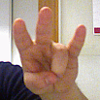
\includegraphics[width=0.15\textwidth]{ChapterFour/1.png}}
    \hfill
    \subfloat{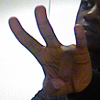
\includegraphics[width=0.15\textwidth]{ChapterFour/4.png}}
    \hfill
    \subfloat{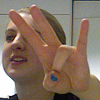
\includegraphics[width=0.15\textwidth]{ChapterFour/3.png}}
    \\\vspace{0.4cm}
    \subfloat{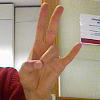
\includegraphics[width=0.15\textwidth]{ChapterFour/2.png}}
    \hfill
    \subfloat{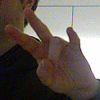
\includegraphics[width=0.15\textwidth]{ChapterFour/5.png}}
    \hfill
    \subfloat{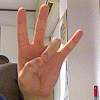
\includegraphics[width=0.15\textwidth]{ChapterFour/6.png}}
    \caption{Inter-signer variability: it is possible to observe not only phonological variations (e.g.\ different handshapes, palm orientations, and sign locations) but also a large physical variability (e.g.\ different hand sizes) when six signers are performing the same sign.}
    \label{fig:inter_signer_variations}
\end{figure}

Borrowing from recent works on adversarial neural networks (\citet{Goodfellow2014, Feutry2018}) and domain transfer (\citet{Ganin2015}), we introduce a deep neural network along with a novel adversarial training objective to specifically tackle the signer-independent SLR problem. The underlying idea is to preserve as much information as possible about the signs, while discarding the signer-specific information that is implicitly present in the manual signing process. For this purpose, the proposed deep model is composed by an \emph{encoder} network, which maps from the input images to latent representations, as well as two discriminative classifiers operating on top of these underlying representations, namely the \emph{sign-classifier} network and the \emph{signer-classifier} network. While the is trained to predict the sign labels, the signer-classifier is trained to discriminate their signer identities. In addition, the parameters of the encoder network are optimized to minimize the loss of the sign-classifier while trying to fool the signer-classifier network. This adversarial and competitive training scheme encourages the learned representations to be signer-invariant and highly discriminative for the sign classification task. To further constrain the latent representations to be signer-invariant, we introduce an additional training objective that operates on the hidden representations of the encoder network in order to enforce the latent distributions of different signers to be as similar as possible.

Although this adversarial training framework is similar to those initially introduced by \citet{Ganin2015}, in the context of domain adaptation, and then by \citet{Feutry2018} to learn anonymized representations, our main contributions on top of these works are two-fold: i) the application of the adversarial training concept to the signer-independent SLR problem and ii) a novel adversarial training objective that differs from the ones of \citet{Ganin2015} and \citet{Feutry2018} in two ways. First, our training objective is minimum if and only if the adversarial classifier, which in our case corresponds to the signer-classifier, produces a uniform distribution over the signer identities, meaning that our model is completely invariant to the signer identity of the training data. Second, we introduce an additional term to the adversarial training objective that further discourages the learned representations of retaining any signer-specific information, by explicitly imposing similarity in the latent distributions of different signers.

The remainder of this section is organized as follows. \Secref{sec:adv_signer_inv_rel_work} presents the related work on SLR. The proposed model along with its adversarial training scheme are fully described in \secref{sec:adv_signer_inv_method}. Experimental results and conclusions are reported in sections~\ref{sec:adv_signer_inv_experiments} and \ref{sec:adv_signer_inv_conclusion}, respectively.

\subsection{Related Work}
\label{sec:adv_signer_inv_rel_work}
We have discussed some of the most relevant approaches for DG in \secref{sec:dg_sota}, so now we shall focus our attention on the specific problem of SLR. This has become an appealing topic in modern society because such systems can ideally be used to reduce the communication barriers that exist between deaf and hearing people.
SLR approaches can be broadly divided into: (i) isolated, which addresses the recognition of single signs either using static images or video (\citet{Marin2014, Marin2016}), and (ii) continuous, which corresponds to the recognition of sentences represented as a sequence of signs (\citet{DanGuo2017, DanGuo2018, Wang2018}). Although most recent works focus on the continuous SLR and its associated problems (e.g.\ large vocabulary size), static SLR is still a challenging task, especially under unconstrained scenarios. One of the biggest challenges is related to the large inter-signer variability, which is in fact the focus of this work.

According to the amount of data required from the test signers, previously signer-independent SLR works can be broadly divided into two main groups: (i) signer adaptation approaches, where a previous trained model is adapted to a new signer by using a small amount of signer specific data, and (ii) truly signer independent methodologies, in which a generic model robust for new test signers is built without using data of those test signers.

The former signer adaptation approaches were greatly inspired by speaker adaptation methods from the speech recognition research. \citet{Agris2006} used maximum likelihood linear regression (MLLR) and maximum a posteriori (MAP) estimation for signer adaptation. In a subsequent work (\citet{Agris2008a}), they extended their work by combining the eigenvoice (EV) approach by \citet{Kuhn2000} with MLLR and MAP to adapt trained hidden Markov models (HMMs) to new signers. MLLR and MAP were the basic adaptation strategies, and the eigenvoice approach provided constraints to reduce the number of free parameters to be adapted. More recently, \citet{Kim2016} investigated the potential of several signer normalization techniques (e.g.\ speed normalization) and different deep neural network adaptation strategies for the signer-independence problem. They found that while signer normalization is ineffective, a simple neural network adaptation strategy, such as fine-tuning the signer-specific neural networks on the adaptation data, is very effective.

The aforementioned methods are all supervised adaptation approaches, in the sense that the adaptation data from the new signer must be labeled. However, in practice, collecting labeled data may be a cumbersome and time-consuming task. To overcome this issue, a few works have resorted to unsupervised adaptation strategies. \citet{Yin2015} proposed a two-step weakly supervised metric learning framework to perform signer adaptation with some unlabeled sign data of the new signer. In the first step, a generic metric is learnt from the available labeled data of several different signers. In the second step, the generic metric is adapted to the new signer by considering clustering and manifold constraints along with the collected unlabeled data.

Although signer adaptation is a reasonable approach, there is still the need to collect either labeled or unlabeled data to retrain and adapt the model for a new signer. Therefore, a truly signer-independent approach, which does not require any data from the new signers, would be the ideal solution for a practical SLR system. Examples of such works can be found are those by \citet{Zieren2005, Shanableh2011, Agris2008b, Kong2014, Kelly2010, Dahmani2014, Yin2016}. Most of them involved a huge feature engineering effort in order to build normalized feature descriptors robust to the physical variations of the signers (e.g.\ height, hand size and length of the arm) and different acquisition conditions (e.g.\ distance to the camera). Afterwards, most of these works use HMMs or their variants for sign recognition. It is the example of the work proposed by \citet{Agris2008b}, in which a set of 11 regional features are extracted (e.g.\ 2-D coordinates, hand blobs area, orientation of the main axis, inertia ratio, eccentricity and compactness) and, then, normalized according to the head position and shoulders distance of the signer. \citet{Kelly2010} introduced a novel signer-independent hand posture feature descriptor, along with an eigenspace size function which represents both qualitative and quantitative properties of a visual shape. \citet{Kong2014} gave particular importance to the movement of epenthesis (ME), which appears as the transition movement that connects successive signs. Concretely speaking, they removed the ME by using a segment and merge approach to decrease the inter-signer variations in ME and used a two-layer Conditional Random Field classifier for sign recognition. More recently, \citet{Yin2016} proposed an interesting and alternative approach that relies on distance metric learning. In particular, the metric is learnt by constraining the distances between the training samples and generic references of the sign classes. The references are constructed by signer invariant representations of each sign class (i.e.\ the average of all samples within the specific class). Afterwards, a two-step iterative optimization strategy is employed to obtain more appropriate references and update the corresponding distance metric alternately.

Although the aforementioned methods have promoted a significant evolution in the signer-independent research, there are still many opportunities for improvement. A major weakness across all the methods is related to the fact that representation and metric learning is not jointly performed. It is well known that the recent success of deep learning approaches, particularly those using CNNs, in tasks like object detection and recognition, has been extended to the SLR problem. The underlying motivation is to automatically learn multiple levels of representations directly from the data (\citet{Pigou2015, Koller2016, Wu2016, Neverova2016, Kumar2017}). However, none of these works explicitly constrains the learned representations to be signer invariant.

\section{Methodology}
\label{sec:adv_signer_inv_methodology}

The ultimate goal of our model is to learn signer-invariant latent representations that preserve the relevant part of the information about the signs while discarding the signer-specific traits that may hamper the sign classification task. To accomplish this purpose, we introduce a deep neural network along with an adversarial training scheme that is able to learn feature representations that combine both sign discriminativeness and signer-invariance.

More specifically, let $\{\mX_{i},y_{i},s_{i}\}_{i=1}^{n}$ be a labeled dataset of $n$ samples, where $\mX_{i}$ represents the $i$-th colour image, and $y_{i}$ and $s_{i}$ denote the corresponding class (sign) label and signer identity, respectively. To induce the model to learn signer-invariant representations, the proposed model comprises three distinct sub-networks:
\begin{itemize}
    \item an encoder network, which aims at learning an encoding function $h(\rmX;\theta_h)$, parameterized by $\theta_h$, that maps from an input image $\rmX$ to a latent representation $\vh$;
    \item a sign-classifier network, which operates on top of this underlying latent representation $\vh$ to learn our task-specific function $f(\vh; \theta_f)$, parameterized by $\theta_f$, that maps from $\vh$ to the predicted probabilities $p(\ry|\vh; \theta_f)$ of each sign class.
    \item a signer-classifier network, with the purpose of learning a signer-specific function $g(\vh; \theta_g)$, parameterized by $\theta_g$, that maps the same hidden representation $\vh$ to the predicted probabilities $p(\rs|\vh;\theta_g)$ of each signer identity.
\end{itemize}

During the learning stage, the parameters of both classifiers are optimized in order to minimize their errors on their specific tasks on the training set. In addition, the parameters of the encoder network are optimized in order to minimize the loss of the sign-classifier network while forcing the signer-classifier to be a random guessing predictor. In the course of this adversarial training procedure, the learned latent representations $\vh$ are encouraged to be signer-invariant and highly discriminative for sign classification. To further discourage the latent representations of retaining any signer-specific traits, we introduce an additional training objective that enforces the latent distributions of different signers to be as similar as possible. The result is a truly signer-independent model robust to new test signers.

\subsubsection{Architecture}
As illustrated in \Figref{fig:model_archi}, the architecture of the proposed model is composed by three main sub-networks or blocks, i.e. an encoder, a sign-classifier, and a signer-classifier.

The encoder network attempts to learn a mapping from an input image $\mX$ to a latent representation $\vz$. It consists of a sequence of $L_{e}$ pairs of consecutive $3\times 3$ convolutional layers with Rectified  Linear  Units (ReLUs) as non-linearities. For downsampling, the last convolutional layer of each pair has a stride of 2. On top of that, there is a fully-connected layer, also with a ReLU, representing the desired signer-invariant latent representations $\vz$.

Taking the latent representations $\vz$ as input, the sign-classifier block is composed by a sequence of $L_{s}$ fully-connected layers, with ReLUs as the non-linear functions, for predicting the sign class $\hat{y} \triangleq \argmax f(\vz; \theta_f)$. Therefore, the last fully-connected layer has a softmax activation function which outputs the probabilities for each sign class.

The signer-classifier network has exactly the same topology as the sign-classifier. However, it maps the latent representations $\vh$ to the predicted signer identity $\hat{s} \triangleq \argmax g(\vz; \theta_g)$. Therefore, the number of nodes of the output layer is defined accordingly to the number of signers in the training set.


\begin{figure*}[t]
\centering
\tikzset{every picture/.style={line width=0.75pt}} %set default line width to 0.75pt

\scalebox{0.6}{










\tikzset{every picture/.style={line width=0.9pt}} %set default line width to 0.75pt

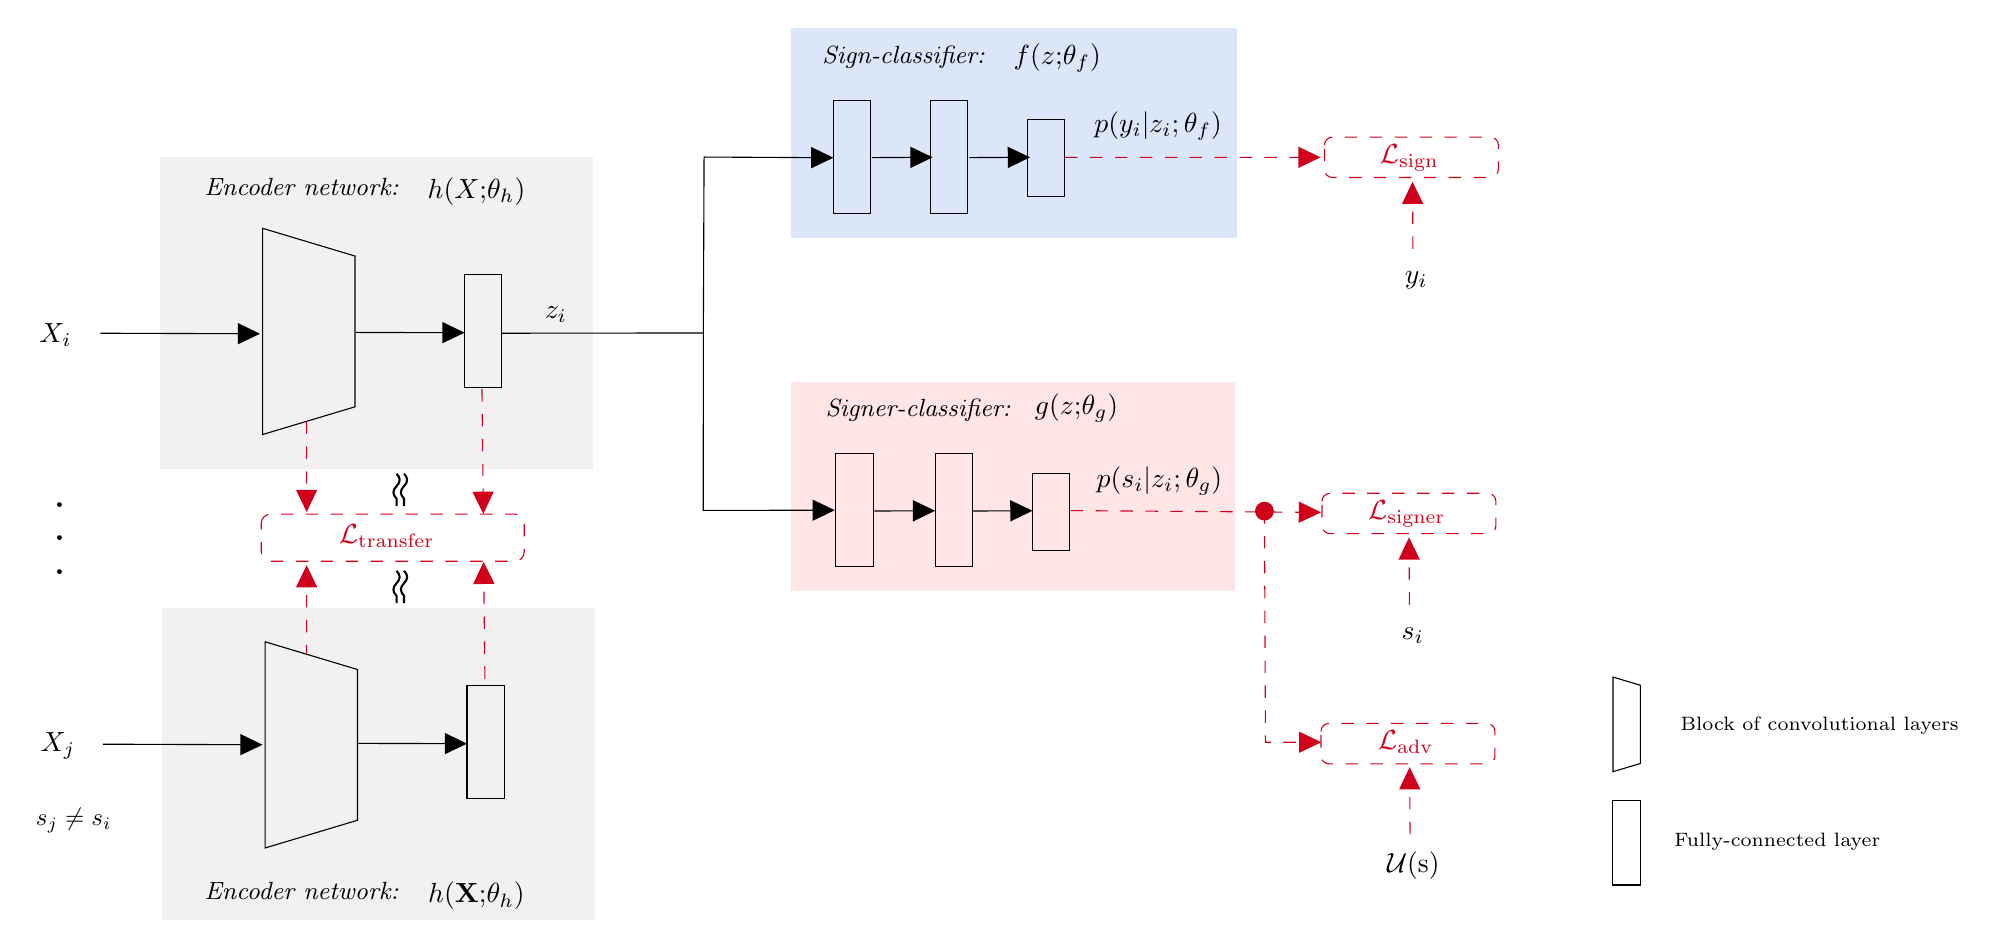
\begin{tikzpicture}[x=0.9pt,y=0.9pt,yscale=-1,xscale=1]
%uncomment if require: \path (0,637); %set diagram left start at 0, and has height of 637

%Shape: Rectangle [id:dp7817430644997849]
\draw  [draw opacity=0][fill={rgb, 255:red, 226; green, 223; blue, 223 }  ,fill opacity=0.46 ][dash pattern={on 4.5pt off 4.5pt}] (89.57,241.83) -- (263.45,241.83) -- (263.45,367) -- (89.57,367) -- cycle ;
%Shape: Rectangle [id:dp43448545781433445]
\draw  [draw opacity=0][fill={rgb, 255:red, 124; green, 163; blue, 233 }  ,fill opacity=0.27 ][dash pattern={on 4.5pt off 4.5pt}] (342,9) -- (521,9) -- (521,93.23) -- (342,93.23) -- cycle ;
%Shape: Rectangle [id:dp47448290384115754]
\draw  [draw opacity=0][fill={rgb, 255:red, 226; green, 223; blue, 223 }  ,fill opacity=0.46 ][dash pattern={on 4.5pt off 4.5pt}] (88.57,60.83) -- (262.45,60.83) -- (262.45,186) -- (88.57,186) -- cycle ;
%Shape: Trapezoid [id:dp7544890433922595]
\draw   (129.83,89.34) -- (166.92,100.47) -- (166.92,161) -- (129.83,172.13) -- cycle ;
%Shape: Rectangle [id:dp07852532899632947]
\draw   (225.83,108) -- (225.83,153.36) -- (210.91,153.36) -- (210.91,108) -- cycle ;
%Straight Lines [id:da6483299081027241]
\draw    (167.27,131.14) -- (208.91,131.24) ;
\draw [shift={(210.91,131.24)}, rotate = 180.14] [fill={rgb, 255:red, 0; green, 0; blue, 0 }  ][line width=0.75]  [draw opacity=0] (8.93,-4.29) -- (0,0) -- (8.93,4.29) -- cycle    ;

%Straight Lines [id:da3383332186453154]
\draw    (64.69,131.46) -- (126.8,131.67) ;
\draw [shift={(128.8,131.68)}, rotate = 180.19] [fill={rgb, 255:red, 0; green, 0; blue, 0 }  ][line width=0.75]  [draw opacity=0] (8.93,-4.29) -- (0,0) -- (8.93,4.29) -- cycle    ;

%Straight Lines [id:da8976159443553993]
\draw    (225.86,131.46) -- (306.79,131.35) ;


%Shape: Rectangle [id:dp39844785350453726]
\draw   (373.93,38.03) -- (373.93,83.38) -- (359.01,83.38) -- (359.01,38.03) -- cycle ;
%Shape: Rectangle [id:dp5960148926786581]
\draw   (412.75,38.03) -- (412.75,83.38) -- (397.84,83.38) -- (397.84,38.03) -- cycle ;
%Shape: Rectangle [id:dp2968748699957451]
\draw   (451.86,45.72) -- (451.86,76.69) -- (436.94,76.69) -- (436.94,45.72) -- cycle ;
%Straight Lines [id:da38135442637321804]
\draw    (374.47,60.94) -- (396.84,60.84) ;
\draw [shift={(398.84,60.83)}, rotate = 539.75] [fill={rgb, 255:red, 0; green, 0; blue, 0 }  ][line width=0.75]  [draw opacity=0] (8.93,-4.29) -- (0,0) -- (8.93,4.29) -- cycle    ;

%Straight Lines [id:da5103446228646831]
\draw    (413.57,60.94) -- (435.94,60.84) ;
\draw [shift={(437.94,60.83)}, rotate = 539.75] [fill={rgb, 255:red, 0; green, 0; blue, 0 }  ][line width=0.75]  [draw opacity=0] (8.93,-4.29) -- (0,0) -- (8.93,4.29) -- cycle    ;

%Shape: Rectangle [id:dp21504155648063916]
\draw  [draw opacity=0][fill={rgb, 255:red, 255; green, 199; blue, 199 }  ,fill opacity=0.46 ][dash pattern={on 4.5pt off 4.5pt}] (342.06,150.9) -- (520.25,150.9) -- (520.25,235.13) -- (342.06,235.13) -- cycle ;
%Shape: Rectangle [id:dp5629086137047858]
\draw   (374.93,179.92) -- (374.93,225.28) -- (360.01,225.28) -- (360.01,179.92) -- cycle ;
%Shape: Rectangle [id:dp11383387176162141]
\draw   (414.75,179.92) -- (414.75,225.28) -- (399.84,225.28) -- (399.84,179.92) -- cycle ;
%Shape: Rectangle [id:dp8834314863600405]
\draw   (453.86,187.61) -- (453.86,218.59) -- (438.94,218.59) -- (438.94,187.61) -- cycle ;
%Straight Lines [id:da7960584409422926]
\draw    (375.47,202.84) -- (397.84,202.74) ;
\draw [shift={(399.84,202.73)}, rotate = 539.75] [fill={rgb, 255:red, 0; green, 0; blue, 0 }  ][line width=0.75]  [draw opacity=0] (8.93,-4.29) -- (0,0) -- (8.93,4.29) -- cycle    ;

%Straight Lines [id:da26603179330471005]
\draw    (414.57,202.84) -- (436.94,202.74) ;
\draw [shift={(438.94,202.73)}, rotate = 539.75] [fill={rgb, 255:red, 0; green, 0; blue, 0 }  ][line width=0.75]  [draw opacity=0] (8.93,-4.29) -- (0,0) -- (8.93,4.29) -- cycle    ;

%Straight Lines [id:da645470302869213]
\draw    (306.79,131.35) -- (307.07,60.72) -- (357,60.99) ;
\draw [shift={(359,61)}, rotate = 180.31] [fill={rgb, 255:red, 0; green, 0; blue, 0 }  ][line width=0.75]  [draw opacity=0] (8.93,-4.29) -- (0,0) -- (8.93,4.29) -- cycle    ;

%Straight Lines [id:da6326177139350364]
\draw    (306.79,131.35) -- (306.74,202.61) -- (357.56,202.5) ;
\draw [shift={(359.56,202.5)}, rotate = 539.88] [fill={rgb, 255:red, 0; green, 0; blue, 0 }  ][line width=0.75]  [draw opacity=0] (8.93,-4.29) -- (0,0) -- (8.93,4.29) -- cycle    ;

%Straight Lines [id:da43094599217232044]
\draw [color={rgb, 255:red, 208; green, 2; blue, 27 }  ,draw opacity=1 ] [dash pattern={on 4.5pt off 4.5pt}]  (452.06,60.88) -- (552.61,60.84) ;
\draw [shift={(554.61,60.83)}, rotate = 539.98] [fill={rgb, 255:red, 208; green, 2; blue, 27 }  ,fill opacity=1 ][line width=0.75]  [draw opacity=0] (8.93,-4.29) -- (0,0) -- (8.93,4.29) -- cycle    ;

%Rounded Rect [id:dp20102262667247417]
\draw  [color={rgb, 255:red, 208; green, 2; blue, 27 }  ,draw opacity=1 ][dash pattern={on 4.5pt off 4.5pt}] (555.16,198.96) .. controls (555.16,197.16) and (556.62,195.71) .. (558.41,195.71) -- (621.75,195.71) .. controls (623.55,195.71) and (625,197.16) .. (625,198.96) -- (625,208.69) .. controls (625,210.48) and (623.55,211.94) .. (621.75,211.94) -- (558.41,211.94) .. controls (556.62,211.94) and (555.16,210.48) .. (555.16,208.69) -- cycle ;
%Straight Lines [id:da7107772326187543]
\draw [color={rgb, 255:red, 208; green, 2; blue, 27 }  ,draw opacity=1 ] [dash pattern={on 4.5pt off 4.5pt}]  (454.25,202.67) -- (552.78,203.37) ;
\draw [shift={(554.78,203.38)}, rotate = 180.41] [fill={rgb, 255:red, 208; green, 2; blue, 27 }  ,fill opacity=1 ][line width=0.75]  [draw opacity=0] (8.93,-4.29) -- (0,0) -- (8.93,4.29) -- cycle    ;

%Straight Lines [id:da7856916848123423]
\draw [color={rgb, 255:red, 208; green, 2; blue, 27 }  ,draw opacity=1 ] [dash pattern={on 4.5pt off 4.5pt}]  (147.5,166.88) -- (147.51,201.24) ;
\draw [shift={(147.51,203.24)}, rotate = 269.99] [fill={rgb, 255:red, 208; green, 2; blue, 27 }  ,fill opacity=1 ][line width=0.75]  [draw opacity=0] (8.93,-4.29) -- (0,0) -- (8.93,4.29) -- cycle    ;

%Straight Lines [id:da899109719860808]
\draw [color={rgb, 255:red, 208; green, 2; blue, 27 }  ,draw opacity=1 ] [dash pattern={on 4.5pt off 4.5pt}]  (217.9,153.87) -- (218.43,202) ;
\draw [shift={(218.45,204)}, rotate = 269.36] [fill={rgb, 255:red, 208; green, 2; blue, 27 }  ,fill opacity=1 ][line width=0.75]  [draw opacity=0] (8.93,-4.29) -- (0,0) -- (8.93,4.29) -- cycle    ;

%Straight Lines [id:da36002582240035363]
\draw [color={rgb, 255:red, 0; green, 0; blue, 0 }  ,draw opacity=1 ][line width=0.75]    (186.6,226.85) .. controls (188.27,228.52) and (188.27,230.18) .. (186.6,231.85) .. controls (184.93,233.52) and (184.93,235.18) .. (186.6,236.85) -- (186.6,239.85) -- (186.6,239.85)(183.6,226.85) .. controls (185.27,228.52) and (185.27,230.18) .. (183.6,231.85) .. controls (181.93,233.52) and (181.93,235.18) .. (183.6,236.85) -- (183.6,239.85) -- (183.6,239.85) ;


%Rounded Rect [id:dp28118263286951617]
\draw  [color={rgb, 255:red, 208; green, 2; blue, 27 }  ,draw opacity=1 ][dash pattern={on 4.5pt off 4.5pt}] (556.16,55.96) .. controls (556.16,54.16) and (557.62,52.71) .. (559.41,52.71) -- (622.75,52.71) .. controls (624.55,52.71) and (626,54.16) .. (626,55.96) -- (626,65.69) .. controls (626,67.48) and (624.55,68.94) .. (622.75,68.94) -- (559.41,68.94) .. controls (557.62,68.94) and (556.16,67.48) .. (556.16,65.69) -- cycle ;
%Straight Lines [id:da5356763271282314]
\draw [color={rgb, 255:red, 208; green, 2; blue, 27 }  ,draw opacity=1 ] [dash pattern={on 4.5pt off 4.5pt}]  (591.52,72.62) -- (591.71,101.6) ;

\draw [shift={(591.51,70.62)}, rotate = 89.63] [fill={rgb, 255:red, 208; green, 2; blue, 27 }  ,fill opacity=1 ][line width=0.75]  [draw opacity=0] (8.93,-4.29) -- (0,0) -- (8.93,4.29) -- cycle    ;
%Straight Lines [id:da9155638065763507]
\draw [color={rgb, 255:red, 208; green, 2; blue, 27 }  ,draw opacity=1 ] [dash pattern={on 4.5pt off 4.5pt}]  (590.12,215.42) -- (590.31,244.4) ;

\draw [shift={(590.11,213.42)}, rotate = 89.63] [fill={rgb, 255:red, 208; green, 2; blue, 27 }  ,fill opacity=1 ][line width=0.75]  [draw opacity=0] (8.93,-4.29) -- (0,0) -- (8.93,4.29) -- cycle    ;
%Straight Lines [id:da7191094178180941]
\draw [color={rgb, 255:red, 0; green, 0; blue, 0 }  ,draw opacity=1 ][line width=0.75]    (186.6,187.85) .. controls (188.27,189.52) and (188.27,191.18) .. (186.6,192.85) .. controls (184.93,194.52) and (184.93,196.18) .. (186.6,197.85) -- (186.6,200.85) -- (186.6,200.85)(183.6,187.85) .. controls (185.27,189.52) and (185.27,191.18) .. (183.6,192.85) .. controls (181.93,194.52) and (181.93,196.18) .. (183.6,197.85) -- (183.6,200.85) -- (183.6,200.85) ;


%Straight Lines [id:da9896530377071313]
\draw [color={rgb, 255:red, 208; green, 2; blue, 27 }  ,draw opacity=1 ] [dash pattern={on 4.5pt off 4.5pt}]  (147.51,226.56) -- (147.5,259.88) ;

\draw [shift={(147.51,224.56)}, rotate = 90.02] [fill={rgb, 255:red, 208; green, 2; blue, 27 }  ,fill opacity=1 ][line width=0.75]  [draw opacity=0] (8.93,-4.29) -- (0,0) -- (8.93,4.29) -- cycle    ;
%Shape: Trapezoid [id:dp6458709768563871]
\draw   (672,269.5) -- (683,272.8) -- (683,304.2) -- (672,307.5) -- cycle ;
%Shape: Rectangle [id:dp1901046474760686]
\draw   (226.83,273) -- (226.83,318.36) -- (211.91,318.36) -- (211.91,273) -- cycle ;
%Straight Lines [id:da8673211689855849]
\draw    (168.27,296.14) -- (209.91,296.24) ;
\draw [shift={(211.91,296.24)}, rotate = 180.14] [fill={rgb, 255:red, 0; green, 0; blue, 0 }  ][line width=0.75]  [draw opacity=0] (8.93,-4.29) -- (0,0) -- (8.93,4.29) -- cycle    ;

%Straight Lines [id:da3618642920648949]
\draw    (65.69,296.46) -- (127.8,296.67) ;
\draw [shift={(129.8,296.68)}, rotate = 180.19] [fill={rgb, 255:red, 0; green, 0; blue, 0 }  ][line width=0.75]  [draw opacity=0] (8.93,-4.29) -- (0,0) -- (8.93,4.29) -- cycle    ;

%Rounded Rect [id:dp5531536926433998]
\draw  [color={rgb, 255:red, 208; green, 2; blue, 27 }  ,draw opacity=1 ][dash pattern={on 4.5pt off 4.5pt}] (129.28,207.86) .. controls (129.28,205.77) and (130.98,204.07) .. (133.07,204.07) -- (231.08,204.07) .. controls (233.17,204.07) and (234.86,205.77) .. (234.86,207.86) -- (234.86,219.21) .. controls (234.86,221.31) and (233.17,223) .. (231.08,223) -- (133.07,223) .. controls (130.98,223) and (129.28,221.31) .. (129.28,219.21) -- cycle ;
%Straight Lines [id:da5399866438305847]
\draw [color={rgb, 255:red, 208; green, 2; blue, 27 }  ,draw opacity=1 ] [dash pattern={on 4.5pt off 4.5pt}]  (218.58,225.21) -- (219.12,273.33) ;

\draw [shift={(218.56,223.21)}, rotate = 89.36] [fill={rgb, 255:red, 208; green, 2; blue, 27 }  ,fill opacity=1 ][line width=0.75]  [draw opacity=0] (8.93,-4.29) -- (0,0) -- (8.93,4.29) -- cycle    ;
%Straight Lines [id:da6744189660599909]
\draw [color={rgb, 255:red, 208; green, 2; blue, 27 }  ,draw opacity=1 ] [dash pattern={on 4.5pt off 4.5pt}]  (532.07,202.88) -- (532.47,295.68) -- (552.87,295.68) ;
\draw [shift={(554.87,295.68)}, rotate = 180] [fill={rgb, 255:red, 208; green, 2; blue, 27 }  ,fill opacity=1 ][line width=0.75]  [draw opacity=0] (8.93,-4.29) -- (0,0) -- (8.93,4.29) -- cycle    ;
\draw [shift={(532.07,202.88)}, rotate = 89.75] [color={rgb, 255:red, 208; green, 2; blue, 27 }  ,draw opacity=1 ][fill={rgb, 255:red, 208; green, 2; blue, 27 }  ,fill opacity=1 ][line width=0.75]      (0, 0) circle [x radius= 3.35, y radius= 3.35]   ;
%Rounded Rect [id:dp27586876312894315]
\draw  [color={rgb, 255:red, 208; green, 2; blue, 27 }  ,draw opacity=1 ][dash pattern={on 4.5pt off 4.5pt}] (554.76,291.36) .. controls (554.76,289.56) and (556.22,288.11) .. (558.01,288.11) -- (621.35,288.11) .. controls (623.15,288.11) and (624.6,289.56) .. (624.6,291.36) -- (624.6,301.09) .. controls (624.6,302.88) and (623.15,304.34) .. (621.35,304.34) -- (558.01,304.34) .. controls (556.22,304.34) and (554.76,302.88) .. (554.76,301.09) -- cycle ;
%Straight Lines [id:da05722319267703546]
\draw [color={rgb, 255:red, 208; green, 2; blue, 27 }  ,draw opacity=1 ] [dash pattern={on 4.5pt off 4.5pt}]  (590.37,307.67) -- (590.56,336.65) ;

\draw [shift={(590.36,305.67)}, rotate = 89.63] [fill={rgb, 255:red, 208; green, 2; blue, 27 }  ,fill opacity=1 ][line width=0.75]  [draw opacity=0] (8.93,-4.29) -- (0,0) -- (8.93,4.29) -- cycle    ;
%Shape: Trapezoid [id:dp41106407745048745]
\draw   (130.83,255.34) -- (167.92,266.47) -- (167.92,327) -- (130.83,338.13) -- cycle ;
%Shape: Rectangle [id:dp5258454923666749]
\draw   (683,319) -- (683,353) -- (671.91,353) -- (671.91,319) -- cycle ;

% Text Node
\draw (46.68,132.11) node   {$\boldsymbol{X}_{i}$};
% Text Node
\draw (48.35,213.89) node  [align=left] {\textbf{{\large .}}\\\textbf{{\large .}}\\\textbf{{\large .}}};
% Text Node
\draw (145.74,72.5) node  [align=left] {{\small \textit{Encoder network:}}};
% Text Node
\draw (215.7,74.44) node   {$h(\boldsymbol{X}\mathrm{;}\mathnormal{\theta _{h}})$};
% Text Node
\draw (387.48,20.66) node  [align=left] {{\small \textit{Sign-classifier:}}};
% Text Node
\draw (448.89,20.95) node   {$f(\boldsymbol{z}\mathrm{;}\mathnormal{\theta _{f}})$};
% Text Node
\draw (393.24,162.34) node  [align=left] {{\small \textit{Signer-classifier:}}};
% Text Node
\draw (456.63,161.64) node   {$g(\boldsymbol{z}\mathrm{;}\mathnormal{\theta _{g}})$};
% Text Node
\draw (589.25,204.03) node   {${\textstyle \mathcal{\textcolor[rgb]{0.82,0.01,0.11}{L}}\textcolor[rgb]{0.82,0.01,0.11}{_{\mathrm{signer}}}}$};
% Text Node
\draw (489.39,48.2) node   {$p( y_{i} |\boldsymbol{z}_{i} ;\mathnormal{\theta _{f}})$};
% Text Node
\draw (247.56,124.01) node   {$\boldsymbol{z}_{i}$};
% Text Node
\draw (179.66,212.92) node   {${\textstyle \mathcal{\textcolor[rgb]{0.82,0.01,0.11}{L}}\textcolor[rgb]{0.82,0.01,0.11}{_{\mathrm{transfer}}}}$};
% Text Node
\draw (590.25,61.03) node   {${\textstyle \mathcal{\textcolor[rgb]{0.82,0.01,0.11}{L}}\textcolor[rgb]{0.82,0.01,0.11}{_{\mathrm{sign}}}}$};
% Text Node
\draw (593,110.17) node   {$y_{i}$};
% Text Node
\draw (591.6,252.97) node   {$s_{i}$};
% Text Node
\draw (47.68,297.11) node   {$\boldsymbol{X}_{j}$};
% Text Node
\draw (145.74,355.5) node  [align=left] {{\small \textit{Encoder network:}}};
% Text Node
\draw (215.7,357.44) node   {$h(\mathbf{X}\mathrm{;}\mathnormal{\theta _{h}})$};
% Text Node
\draw (588.85,295.43) node   {${\textstyle \mathcal{\textcolor[rgb]{0.82,0.01,0.11}{L}}\textcolor[rgb]{0.82,0.01,0.11}{_{\mathrm{adv}}}}$};
% Text Node
\draw (591.85,345.22) node   {$\mathcal{U}(\mathrm{s})$};
% Text Node
\draw (755,289) node  [align=left] {{\scriptsize Block of convolutional layers}};
% Text Node
\draw (738,335.5) node  [align=left] {{\scriptsize Fully-connected layer}};
% Text Node
\draw (53.96,327) node [scale=0.9]  {$\mathnormal{s_{j} \neq s_{i}}$};
% Text Node
\draw (489.89,190.7) node   {$p( s_{i} |\boldsymbol{z}_{i} ;\mathnormal{\theta _{g}})$};


\end{tikzpicture}




}

\caption{The architecture of the proposed signer-invariant neural network. It comprises three main sub-networks or blocks, i.e. an \textit{encoder}, a \textit{sign-classifier} and a \textit{signer-classifier}.}
\label{fig:model_archi}
\end{figure*}


\subsubsection{Adversarial training}
By definition, signer-invariant representations discard all signer-specific information and, as such, no function (i.e.\ classifier) exists that maps such representations into the correct signer identity. This naturally leads to an adversarial problem, in which: (i) a signer-classifier network $g(\bcdot; \theta_g)$ receives latent representations $\vz \triangleq h(\rmX;\theta_h)$ from an encoder network $h(\bcdot;\theta_h)$ and tries to predict the signer identity $s$ corresponding to image $\mX$ and (ii) the encoder network tries to fool the signer-classifier network while still providing good representations for the sign-classifier network $f(\bcdot; \theta_f)$, which in turn receives the same representations $\vz$ and aims to predict the sign label $y$ corresponding to image $\mX$.

Therefore, the signer-classifier network shall be trained to minimize the negative log-likelihood of correct signer predictions:
\begin{equation}
\label{eq:signer_loss}
\min_{\theta_g} \; \left\lbrace \gL_{\text{signer}}(\theta_h, \theta_g) \triangleq -\frac{1}{n}\sum_{i=1}^n \log p(s_i \mid h(\mX_{i}; \theta_h); \theta_g) \right\rbrace
\end{equation}

In the perspective of the encoder, the predictions of the sign-classifier should be as accurate as possible and the predictions of the signer-classifier should be kept close to uniform, meaning that this latter model is not capable of doing better than random guessing the signer identity. Formally, this may be translated into the following constrained objective:
\begin{align}
\label{eq:sign_loss}
&\min_{\theta_h, \theta_f} \; \left\lbrace \gL_{\text{sign}}(\theta_h, \theta_f)\triangleq-\frac{1}{n}\sum_{i=1}^n \log p(y_i \mid h(\mX_{i}; \theta_h); \theta_f)\right\rbrace,\\
\label{eq:kl_obj}
&\text{subject to } \; \frac{1}{n}\sum_{i=1}^n \KL(\gU(\rs) || p(\rs \mid h(\mX_{i}; \theta_h); \theta_g) \leq \epsilon,
\end{align}
where $\KL$ is the Kullback-Leibler (KL) divergence and $\gU_{\sS}(\rs)$ denotes the discrete uniform distribution on the random variable $\rs$, defined over the set of signer identities $\{1, 2, \dots, k\}$ in the training set. Here, $\epsilon \geq 0$ determines how far from uniform the signer-classifier predictions are allowed to be (as measured by the KL divergence). The choice of the uniform distribution implies the underlying assumption that the training set is balanced relatively to the number of examples per signer (which should be true for most practical datasets). When this is not the case, the empirical distribution of signer identities in the training set may be used instead.

The inequality constraint~\plaineqref{eq:kl_obj} may be rewritten as:
\begin{equation}
\label{eq:adv_loss}
\gL_{\text{adv}}(\theta_h, \theta_g) \triangleq \frac{1}{nk}\sum_{i=1}^n \sum_{\rs} \log p(\rs \mid h(\mX_{i}; \theta_h); \theta_g) \leq \epsilon + \log k,
\end{equation}
and the constrained optimization problem may be equivalently formulated as:
\begin{equation}
\label{eq:tr_obj}
\min_{\theta_h, \theta_f}  \left\lbrace \gL(\theta_h, \theta_f, \theta_g) \triangleq \gL_{\text{sign}}(\theta_h, \theta_f) + \mu_d \gL_{\text{adv}}(\theta_h, \theta_g) \right\rbrace,
\end{equation}
where $\mu_d \geq 0$ depends on $\epsilon$ and $\gL_{\text{adv}}$ plays the role of an adversarial loss with respect to the signer classification loss $\gL_{\text{signer}}$.

This objective and the structure of our model are similar to those used by \citet{Ganin2015}, in the context of domain adaptation, and by \citet{Feutry2018}, to learn anonymized representations for privacy purposes. However, the former uses the negative signer classification loss as the adversarial term (i.e.\ $\gL_{\text{adv}} \leftarrow -\gL_{\text{signer}}$), which is not lower bounded, leading to high gradients and more difficult optimization. The latter addresses this problem by replacing this term with the absolute difference between the adversarial loss as defined in \eqref{eq:adv_loss} and the signer classification loss (i.e.\ $\gL_{\text{adv}} \leftarrow |\gL_{\text{adv}} - \gL_{\text{signer}}|$). This option has a nice information theoretic interpretation as being an empirical upper-bound for the mutual information between the distribution of signer identities and the distribution of latent representations. Nonetheless, there exist infinitely many (non-uniform) distributions for which this loss vanishes. Our choice, besides being clearly lower bounded by the entropy of the uniform distribution, $\log k$, is minimum if and only if $p(\rs \mid h(\mX_{i}; \theta_h); \theta_g) \equiv \gU(\rs)$, $\forall i$, meaning that the signer-classifier block is completely agnostic relatively to the signer identities of the training samples.

\subsubsection{Signer-transfer training objective}
To further encourage the latent representations $\vh$ to be signer-invariant, we introduce an additional term in objective~\plaineqref{eq:tr_obj}, the so-called signer-transfer loss $\gL_{\text{transfer}}$. The core idea of $\gL_{\text{transfer}}$ is to enforce the latent distributions of different signers to be as similar as possible. In practice, this is achieved by minimizing the difference between the hidden representations of different signers, at each layer of the encoder network. To measure the signers distribution difference at the $l$-th layer, $l \in \{1,...,m\}$, we compute a distance $\gD^{(m)}$ between the hidden representations $h^{(l)}(\bcdot;\theta_h)$ of two signers $s$ and $t$ at the output of that layer, as:
\begin{equation}
\label{eq:sign_transfer_pairwise_loss}
\gD^{(l)}(s, t; \theta_h) \triangleq \Big|\Big| \frac{1}{n_s} \sum_{\substack{i: s_i = s}} h^{(m)}(\mX_{i}; \theta_h) - \frac{1}{n_t}\sum_{\substack{j: s_j = t}} h^{(m)}(\mX_{j}; \theta_h) \Big|\Big|_2^2,
\end{equation}
where $||\bcdot||_2$ is the $\normltwo$-norm, and $n_s$ and $n_t$ denote the number of training examples of signers $s$ and $t$, respectively. Accordingly, the signer-transfer loss at the $m$-th layer is the sum of the pairwise distances between all signers, i.e.:
\begin{equation}
\gL_{\text{transfer}}^{(l)}(\theta_h) \triangleq \sum_{s = 1}^k \sum_{\substack{t=1 \\ t \neq s}}^k \gD^{(l)}(s,t; \theta_h)
\end{equation}
The overall signer-transfer loss $\gL_{\text{transfer}}$ is then a weighted sum of the losses computed at each layer of the encoder network, such that:
\begin{equation}
\label{eq:signer_transfer_loss}
\gL_{\text{transfer}}(\theta_h) = \sum_{l=1}^{m}~\beta^{(l)}~\gL_{\text{transfer}}^{(l)}(\theta_h),
\end{equation}
where $\beta^{(l)}\geq 0$ is a hyperparameter that controls the relative importance of the loss obtained at the $l$-th layer.
By combining \plaineqref{eq:tr_obj} and \plaineqref{eq:signer_transfer_loss}, the encoder and sign-classifier networks are trained to minimize the following loss function:
\begin{equation}
\label{eq:enc_sign_loss}
\min_{\theta_h, \theta_f} \left\lbrace \gL(\theta_h, \theta_f, \theta_g) \triangleq \gL_{\text{sign}}(\theta_h, \theta_f) + \mu_d \gL_{\text{adv}}(\theta_h, \theta_g) +
\mu_t \gL_{\text{transfer}}(\theta_h) \right\rbrace,
\end{equation}
where $\mu_t \geq 0$ is the weight that controls the relative importance of the signer-transfer term.

Summing up, the adversarial training procedure is organized by alternating between the minimization of objective~\plaineqref{eq:enc_sign_loss} and the minimization of objective~\plaineqref{eq:signer_loss}.

\subsection{Experimental evaluation}
\label{sec:adv_signer_inv_experiments}

%\subsection{Datasets and evaluation protocol}
\hspace{\parindent}The experimental evaluation of the proposed model was performed using two publicly available SLR databases: the Jochen-Triesch database (\citet{Triesch2001}), and the Microsoft Kinect and Leap Motion American sign language (MKLM) database (\citet{Marin2014, Marin2016}).
Jochen-Triesch is a dataset of 10 hand signs performed by 24 signers against three different types of backgrounds: uniform light, uniform dark and complex. Experiments on this dataset were conducted using its standard evaluation protocol (\citet{Just2006}), in which 8 signers are used for the training and the remaining 16 signers are used for the test. MKLM contains a total of 10 signs, each one repeated 10 times by 14 different signers. In this dataset, the performance of the models is assessed using 5 random splits, created with signer-independence, yielding at each split a training set of 10 signers, a validation set of 2 signers and a test set of 2 signers.

\subsubsection{Implementation details}
In order to extract the manual signs from the noisy background of the images, the automatic hand detection algorithm \cite{Ferreira2018} is used as a pre-processing step. The images are then cropped, resized to the average sign size of the training set, and normalized to be in the range $[-1,1]$.

Throughout this section, the proposed model is compared with state-of-the-art methods for each dataset. Nevertheless, to further attest the robustness of the proposed model, two different baselines are also implemented:
\begin{itemize}
    \item (Baseline 1) A CNN trained from scratch with $\normltwo$ regularization. For a fair comparison, the architecture of the baseline CNN corresponds to the architecture of the encoder network followed by the sign-classifier network of the proposed model.
    \item (Baseline 2) A CNN with the baseline 1 topology, but trained with the triplet loss (\citet{Schroff2015}).
\end{itemize}
Here, the triplet loss concept is explored in order to impose signer-independence in the representation space and, hence, build up a more robust baseline. The underlying idea is to minimize the distance between an \textit{anchor} and a \textit{positive} latent representation, $\vh_{y_{i}, s_{i}}$ and $\vh_{y_{p}, s_{p}}$, respectively; while maximizing the distance between the anchor $\vh_{y_{i}, s_{i}}$ and a \textit{negative} representation $\vh_{y_{n}, s_{n}}$. It is important to note that while anchor and positive latent representations have to be from the same sign class, their signer identity may or not change. On the other hand, anchor and negative representations are from different sign classes, whereas their signer identity may also change. In order to train baseline 2 in an end-to-end fashion for sign classification, the overall loss function to be minimized is a trade-off between the triplet loss $\mathcal{L}_{\text{triplet}}$, defined below, and the classification loss $\mathcal{L}_{\text{sign}}$:
\begin{equation}
\mathcal{L}_{\text{triplet}} \triangleq \frac{1}{n}\sum_{i=1}^{n}\Big[||\vh_{y_{i}, s_{i}}-\vh_{y_{p}, s_{p}}||^2_2 - ||\vh_{y_{i}, s_{i}}-\vh_{y_{n}, s_{n}}||^2_2 + \alpha\Big],
\end{equation}
where $y_{p}=y_{i}$ and $y_{n}\neq$ and the margin $\alpha$ enforced between \emph{positive} and \emph{negative} pairs was fixed at $\alpha=1$. In addition, following \citet{Schroff2015}, an \emph{online} triplet generation strategy, by selecting the hardest positive/negative samples within every mini-batch, was adopted. The overall loss for this model is therefore $\mathcal{L}_{\text{sign}} + \rho \mathcal{L}_{\text{triplet}}$, where $\rho \geq 0$ is a hyperparameter.

All deep models were implemented in PyTorch and trained with the Adam optimization algorithm using a batch size of 32 samples. For reproducibility purposes, the source code as well as the weights of the trained models are publicly available online\footnote{\url{https://github.com/pmmf/SI-SLR}}. The hyperparameters that are common to all the implemented models (i.e.\ learning rate and $\normltwo$ regularization weight) as well as some hyperparameters that are specific to the proposed model (i.e.\ $\mu_d$ and $\mu_t$) and to the implemented baseline~2 (i.e.\ $\rho$) were optimized by means of a grid search approach and cross-validation on the training set (see \Tableref{tab:hyper} for more details).
The signer-transfer penalty $\gL_{\text{transfer}}$ is applied to the last two layers of the encoder network with a relative weight of 1. Regarding the model architecture, the number of consecutive convolutional layers pairs $L_{e}$ was set to 3, which results in a total of 6 convolutional layers. The number of filters starts as 32 which is then doubled after each convolutional pair. The dense layer on top of the encoder network has 128 neurons. The number of dense layers of both classifiers $L_{s}$ was set to 3, and the number of nodes of each hidden layer was set as 128.

\begin{table}[t]
    \centering

    \label{tab:hyper}
    \resizebox{0.5\columnwidth}{!}{
        \begin{tabular}{c|c|c}
            Hyperparameters                    & Symbol & Set                \\ \hline
            Leaning rate                                & --      & \{$1\text{e}^{-04}$,$1\text{e}^{-03}$\}             \\
            $\normltwo$-norm coefficient                              & --       & \{$1\text{e}^{-05}$,$1\text{e}^{-04}$\}             \\
            $\mathcal{L}_{\text{triplet}}$ weight                 & $\rho$                & \{0.1,0.5,1,5,10\}                  \\
            $\mathcal{L}_{\text{adv}}$ weight                 & $\mu_d$                & \{0.1,0.5,0.8,1,3\}                  \\
            $\mathcal{L}_{\text{transfer}}$ weight                 & $\mu_t$                & \{$1.5\text{e}^{-04}$,$2\text{e}^{-04}$,$4\text{e}^{-04}$,$1\text{e}^{-03}$\}                  \\
        \end{tabular}
    }
    \caption{Hyperparameters sets.}
\end{table}

\subsubsection{Results and discussion}
Experiments on the Jochen-Triesch and MKLM databases are summarized in Tables~\ref{tab:joint_table}(a) and ~\ref{tab:joint_table}(b), respectively. We compare our method with other state-of-the-art approaches that have published results on these datasets (\citet{Dahmani2014, Just2006, Kelly2010, Marin2014, Ferreira2018}). The results on the Jochen-Triesch database are presented in terms of average classification accuracy in the overall test set as well as against each specific background type (i.e.\ uniform and complex). For the MKLM database, \Tableref{tab:joint_table}(b) depicts the average classification accuracy computed across all the 5 test splits, as well as the minimum and maximum accuracy value achieved by each method.

\begin{table}[t]
    \centering
    \resizebox{1\textwidth}{!}{
        \begin{tabular}{cc}

            \begin{tabular}{c|c c c}
                & \multicolumn{3}{c}{Background}                \\
                & Uniform        & Complex         & Both          \\ \hline
                \citet{Just2006}       & 92.79           & 81.25           & 87.92         \\
                \citet{Kelly2010} & 91.80            & --               & --             \\
                \citet{Dahmani2014} & 93.10            & --               & --             \\ \hline
                CNN (Baseline 1)                            & 97.50           & 74.38           & 89.79         \\
                CNN with Triplet loss (Baseline 2)          & 98.13           & 75.63           & 90.63              \\
                Proposed method       &      \textbf{98.75}     & \textbf{ 91.25}
                &   \textbf{96.25}     \\
            \end{tabular}

            &

            \begin{tabular}{c|c c c}
                & Average (std)  & min         & max \\ \hline
                \citet{Marin2014}       & 89.71 ( -- )             & --                    & --            \\
                \citet{Ferreira2018} & 93.17 ( -- )             & --                    & --            \\\hline
                CNN (Baseline 1)                              & 89.90 (8.81)            & 73.00                & 98.00        \\
                CNN with Triplet loss (Baseline 2)            & 91.40 (3.93)            & 86.50                & 96.50        \\
                Proposed method        &    \textbf{94.80 (3.53)}      &   \textbf{89.50}
                &  \textbf{100.00}       \\
            \end{tabular} \\

            (a) Jochen-Triesch & (b) MKLM \\
        \end{tabular}}
        \caption{Classification accuracy (\%) on (a) Jochen-Triesch and (b) MKLM datasets.}
        \label{tab:joint_table}
\end{table}

The most relevant observation is the superior performance of the proposed model. Specifically, the proposed model provides the best overall classification accuracy on both SLR databases, clearly outperforming both implemented baselines and all the previous state-of-the-art models. In complex scenarios, as reported in \Tableref{tab:joint_table}(a), the proposed model surpasses all the other methods by a large margin. In addition, by analyzing the standard deviation as well as the minimum and maximum accuracy values, it possible to observe that the proposed model is the method with the lowest variability, yielding consistently high accuracy rates across all test splits of the MKLM dataset (see \Tableref{tab:joint_table}(b)). These results attest the robustness of the proposed model and its capability of better dealing with the large inter-signer variability that exists in the manual signing process of sign languages. Interestingly, the obtained results also reveal that the implemented baselines are in fact fairly strong models, both of them outperforming most of the state-of-the-art methods on both datasets.

\Tableref{tab:loss_terms} illustrates the effect of each proposed training scheme by itself. For this purpose, the proposed model was trained either (i) with just the adversarial procedure, without the signer-transfer $\gL_{\text{transfer}}$ loss, or (ii) with just the $\gL_{\text{transfer}}$ penalty on the encoder network without adversarial training. The results clearly demonstrate the complementary effect between the two training procedures, as their combination provides the best overall classification accuracy. Interestingly, each training scheme outperforms on its own both baselines and state-of-the-art methods.

\begin{table}[t]
    \centering
    \resizebox{0.55\columnwidth}{!}{
        \begin{tabular}{c|c c c }
            & Adversarial ($\gL_{\text{adv}}$) only  & Signer-transfer ($\gL_{\text{transfer}}$) only & Both \\ \hline
            Jochen-Triesch                              & 95.21            & 94.38                & \textbf{96.25}        \\
            MKLM            & 94.00            & 94.10                & \textbf{94.80}        \\
        \end{tabular}
    }
    \caption{\centering The effect of each training procedure in the proposed model. The results in the last column are replicated from Tables~\ref{table:joint_table}(a) and \ref{table:joint_table}(b) as they include both training procedures.}
    \label{tab:loss_terms}
\end{table}

\subsubsection{Latent space visualization}
To further demonstrate the effectiveness of the proposed model in promoting signer-invariant latent representation spaces, we show in \Figref{fig:adv_signer_inv_tsne} a visual inspection of the latent representations through the t-distributed stochastic neighbor embedding (t-SNE, \citet{Maaten2008}). These plots clearly demonstrate the better capability of the proposed model of imposing signer-independence in the latent representations. The proposed model yields a latent representation space in which representations of different signers and same class are close to each other and well mixed, while it keeps latent representations of different classes far apart. By analyzing the t-SNE plot of baseline~1, it is possible to observe that the latent representations of different signers and the same class tend to be far apart in the latent space. In addition, there is some overlapping between clusters of different classes. Although baseline~2 (CNN with the triplet loss) promoted slightly improvements over the standard baseline CNN, the proposed model achieved by far the best signer-invariance and class separability.

\begin{figure}
    \resizebox{1\textwidth}{!}{
        \setlength\tabcolsep{1pt}
        \begin{tabular}{ccc}
            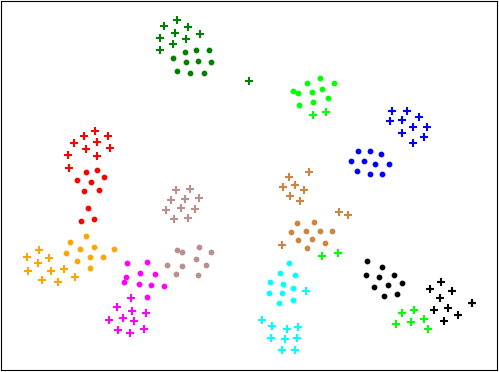
\includegraphics[width=0.325\textwidth]{ChapterFour/tsne_baseline.png} &
            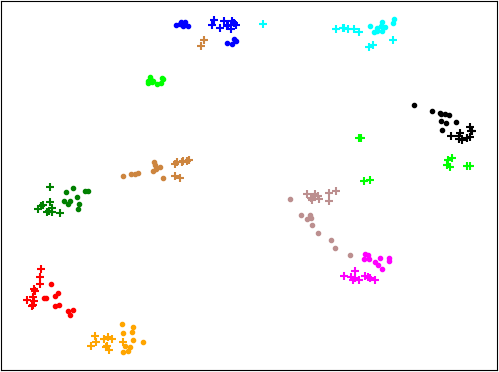
\includegraphics[width=0.325\textwidth]{ChapterFour/tsne_triplet.png} &
            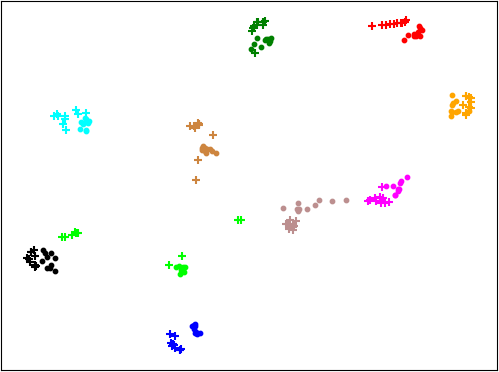
\includegraphics[width=0.325\textwidth]{ChapterFour/tsne_proposed.png}\\
            \footnotesize{(a) CNN - baseline 1} & \footnotesize{(b) CNN with triplet loss - baseline 2} & \footnotesize{(c) Proposed model}
        \end{tabular}
    }
    \caption{\centering Two-dimensional projection of the latent representation space using the t-distributed stochastic neighbor embedding (t-SNE). Markers $\bullet$ and $\textbf{+}$ represent 2 different test signers, while the different colors denote the 10 sign classes.}
    \label{fig:adv_signer_inv_tsne}
\end{figure}

%-------------------------------------------------------------------------
\subsection{Conclusion}
\label{sec:adv_signer_inv_conclusion}

This paper presents a novel adversarial training objective, based on representation learning and deep neural networks, specifically designed to tackle the signer-independent SLR problem. The underlying idea is to learn signer-invariant latent representations that preserve as much information as possible about the signs, while discarding the signer-specific traits that are irrelevant for sign recognition. For this purpose, we introduce  an adversarial training procedure for simultaneously training an \textit{encoder} and a \textit{sign-classifier} over the target sign variables, while preventing the latent representations of the \textit{encoder} to be predictive of the signer identities. To further discourage the underlying representations of retaining any signer-specific information, we propose an additional training objective that enforces the latent distributions of different signers to be as similar as possible.
Experimental results demonstrate the effectiveness of the proposed model in several SLR databases.
